% The x³−2 mod 5 example: the tower ℚ(∛2,ω)/ℚ(∛2)/ℚ with primes and
% the matching factorizations of x³−2 at each level.
% Source: book/tex/alg-NT/frobenius.tex (§ Frobenius controls
% polynomial factorization) — tikzcd.
\documentclass[border=2mm]{standalone}
\usepackage{tikz}
\usepackage{amssymb}
\usepackage{amsmath}
\begin{document}
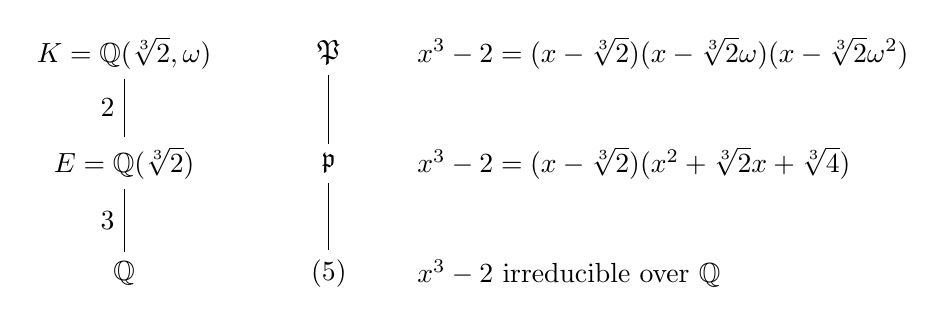
\begin{tikzpicture}
  \node (K)  at (0,2.8)    {$K = \mathbb{Q}(\sqrt[3]{2}, \omega)$};
  \node (E)  at (0,1.4)    {$E = \mathbb{Q}(\sqrt[3]{2})$};
  \node (Q)  at (0,0)      {$\mathbb{Q}$};
  \node (PP) at (2.6,2.8)  {$\mathfrak{P}$};
  \node (pp) at (2.6,1.4)  {$\mathfrak{p}$};
  \node (p)  at (2.6,0)    {$(5)$};
  \node[anchor=west] (f1) at (3.6,2.8) {$x^3-2 = (x-\sqrt[3]{2})(x-\sqrt[3]{2}\omega)(x-\sqrt[3]{2}\omega^2)$};
  \node[anchor=west] (f2) at (3.6,1.4) {$x^3-2 = (x-\sqrt[3]{2})(x^2+\sqrt[3]{2}x+\sqrt[3]{4})$};
  \node[anchor=west] (f3) at (3.6,0)   {$x^3-2$ irreducible over $\mathbb{Q}$};
  \draw (K) -- (E) node[midway,left] {$2$};
  \draw (E) -- (Q) node[midway,left] {$3$};
  \draw (PP) -- (pp) -- (p);
\end{tikzpicture}
\end{document}
